\documentclass[a4paper]{article}
\usepackage[letterpaper, margin=1in]{geometry} % page format
\usepackage{listings} % this package is for including code
\usepackage{graphicx} % this package is for including figures
\usepackage{amsmath}  % this package is for math and matrices
\usepackage{amsfonts} % this package is for math fonts
\usepackage{hyperref} % for urls
\usepackage{cite}

\title{Homework 01}
\date{2013-09-20}
\author{Morgan Baker}
\begin{document}
\lstset{language=Python}
	
\maketitle

\section{Solution to Section 1.4}
\subsection{Solution to Part A}
Part A states that we need to set up a linearly separable data set with size 20.  There is a webstie for this that professor Rivas recommended we use. This website is found at The Data Science Lab\cite[]{citation01}. The code from this website is saved in the baker-01 folder as Perceptron.py. After importing this class, there was one edit I had to make. The edit was to import the pyplot class from matplotlib as plt. The result of this is \ref {fig:PartA}


\begin{figure}
  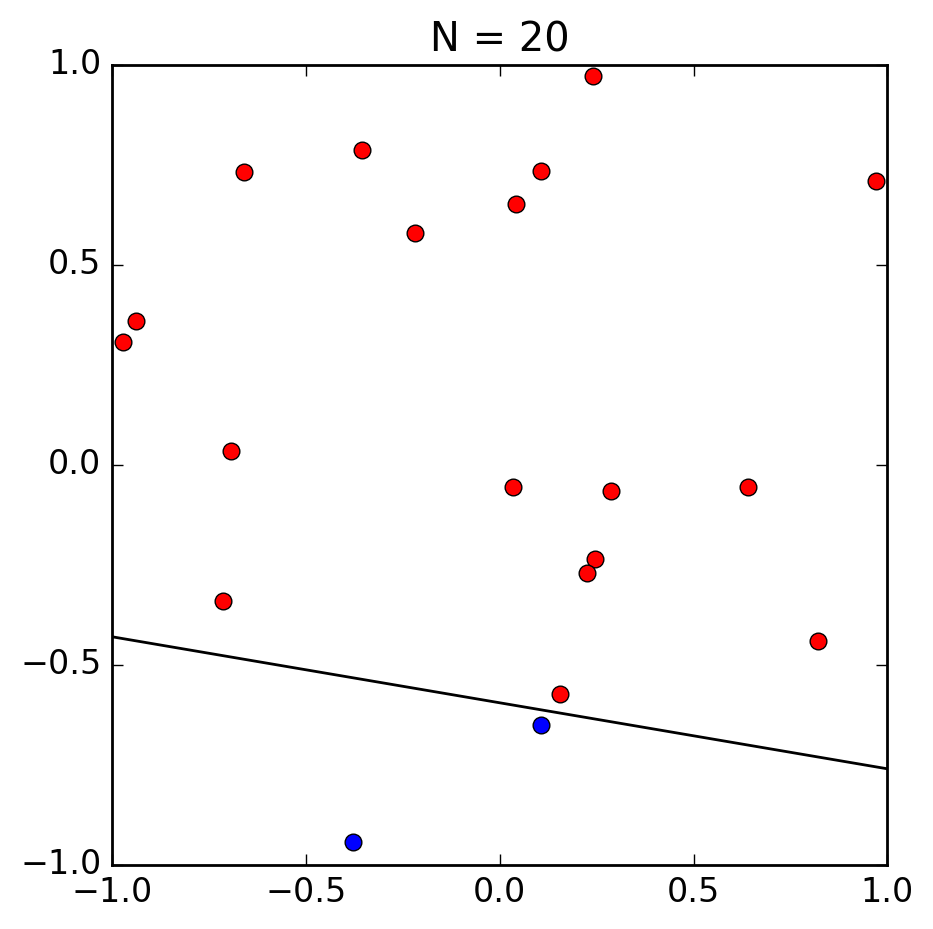
\includegraphics[width=9cm,height=9cm]{p_N20.png}
  \caption{Part A plot with target function f.}
  \label{fig:PartA}
\end{figure}

\subsection{Solution to Part B}
Part B states that we need to run the perceptron learning algorithm on the plot from part A. The code uses the pla method from the Perceptron class. Included are three iterations of the algorithm running. The first picture, \ref{fig:PartB1}, is the first iteration that was clearly visible on the plot. The second picture, \ref{fig:PartB2}, is much closer to the target function than the first picture, but still not there yet. The last picture, \ref{fig:PartB3}, is when the algorithm stopped. While the hypothesis g is close to the function f, the slope is visibily off. 

\begin{figure}
  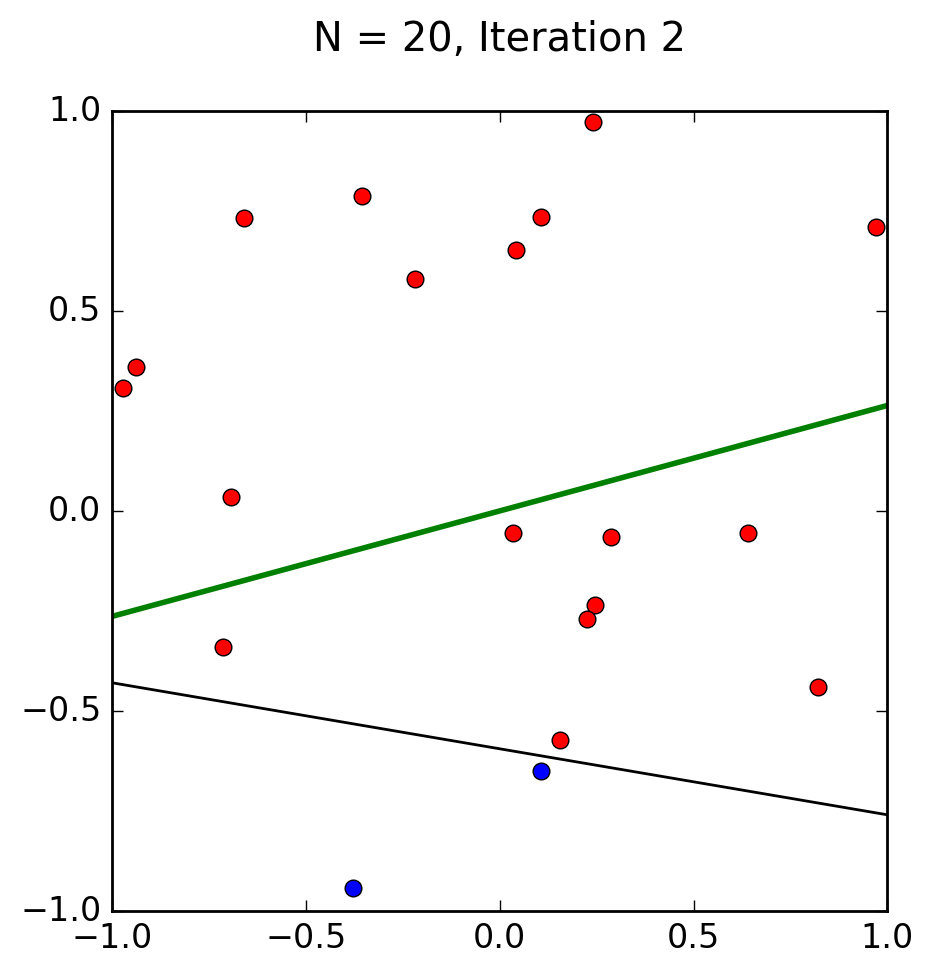
\includegraphics[width=9cm,height=9cm]{p_N20_it2.png}
  \caption{An iteration of the perceptron learning algorithm.}
  \label{fig:PartB1}
\end{figure}
\begin{figure}
  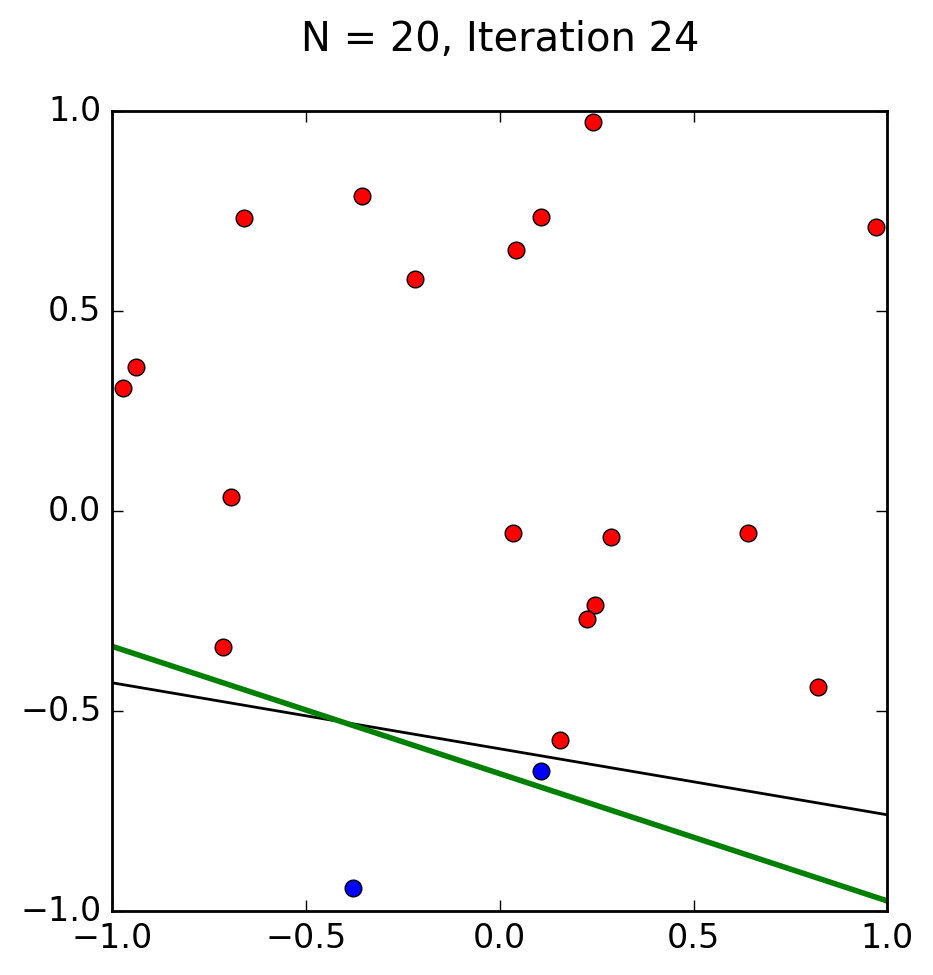
\includegraphics[width=9cm,height=9cm]{p_N20_it24.png}
  \caption{An iteration of the perceptron learning algorithm.}
  \label{fig:PartB2}
\end{figure}
\begin{figure}
  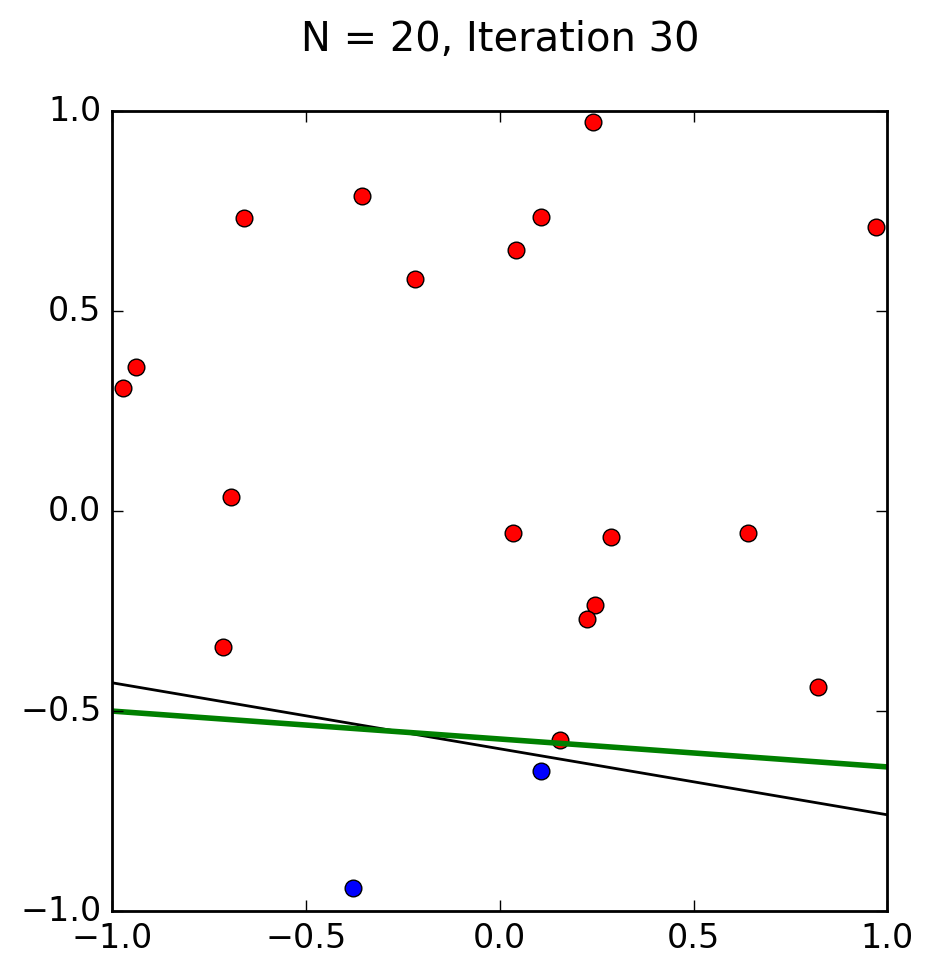
\includegraphics[width=9cm,height=9cm]{p_N20_it30.png}
  \caption{The last iteration of the perceptron learning algorithm.}
  \label{fig:PartB3}
\end{figure}

\subsection{Solution to Part C}
Part C states that we need to run the perceptron learning algorithm on a different set of 20 points. The code uses the pla method from the Perceptron class. Included are three iterations of the algorithm running. The first picture, \ref{fig:PartC1}, is one of the iterations that got close. The second picture, \ref{fig:PartC2}, is the iteration after the first picture. This was a little weird to see. The last picture, \ref{fig:PartC3}, is when the algorithm stopped. While the hypothesis g is close to the function f, the slope is visibily off, just like the function in Part B.
\begin{figure}
  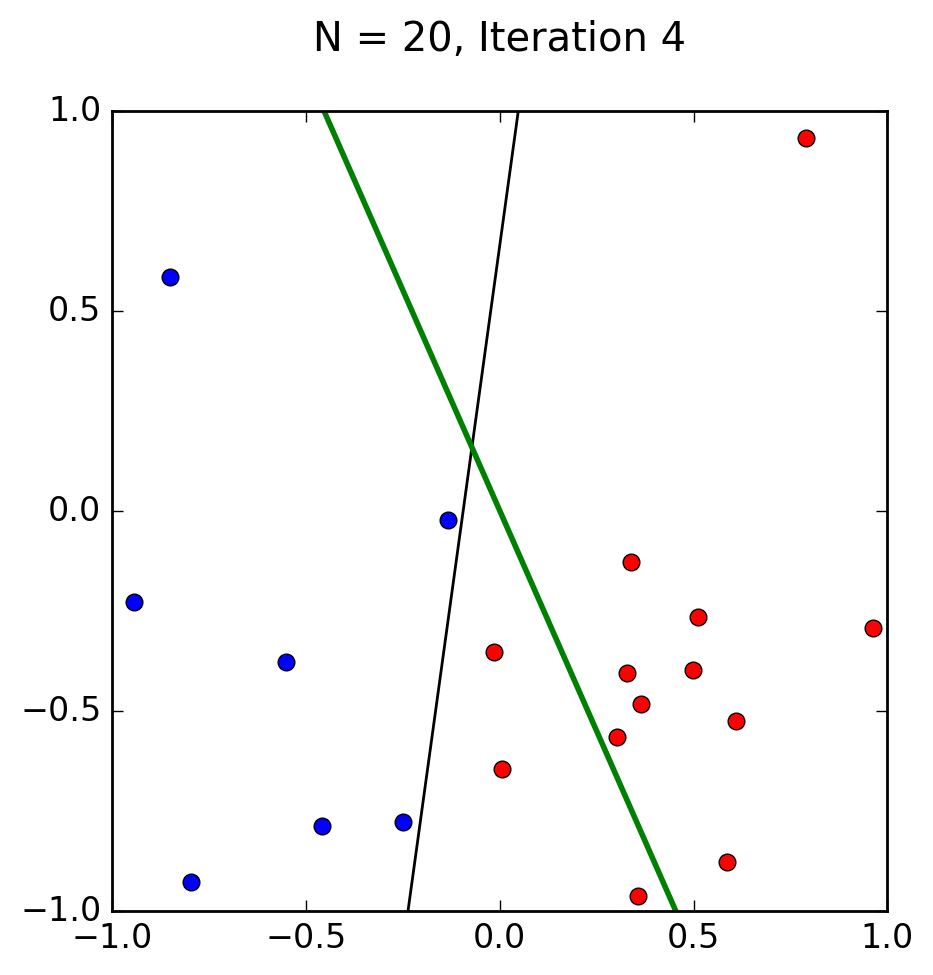
\includegraphics[width=9cm,height=9cm]{p_N20_it4.png}
  \caption{An iteration of the perceptron learning algorithm.}
  \label{fig:PartC1}
\end{figure}
\begin{figure}
  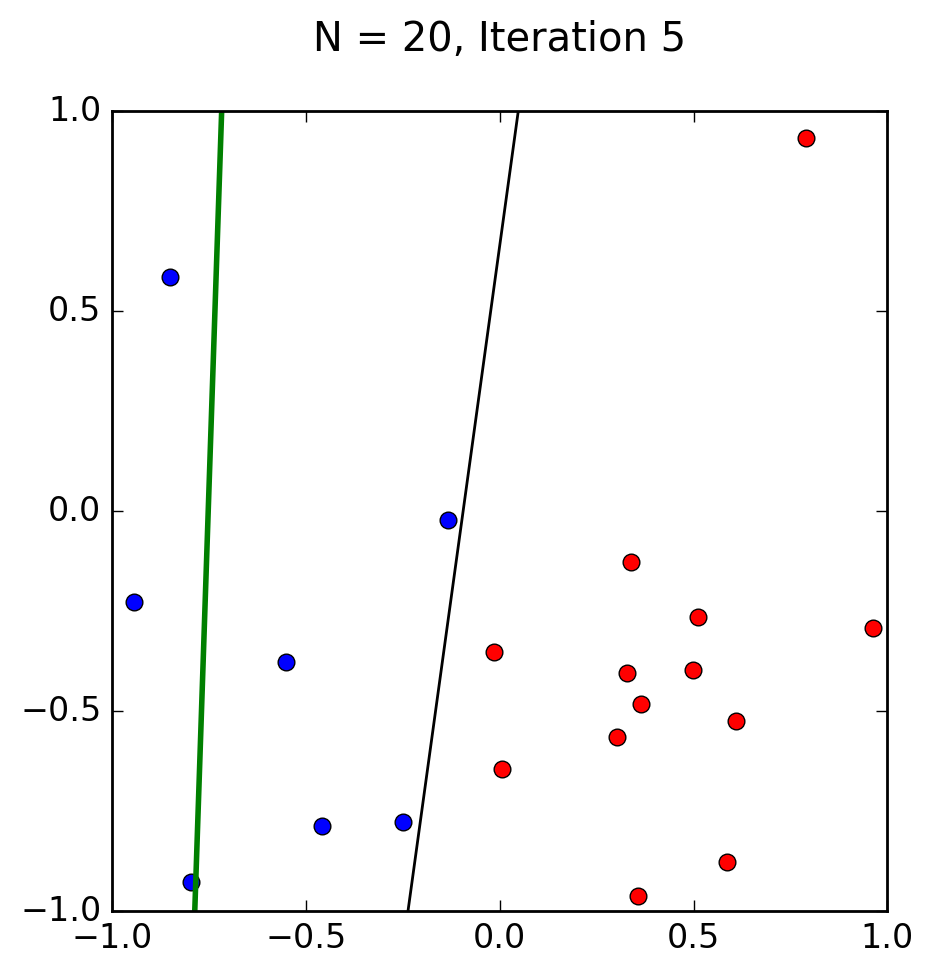
\includegraphics[width=9cm,height=9cm]{p_N20_it5.png}
  \caption{An iteration of the perceptron learning algorithm.}
  \label{fig:PartC2}
\end{figure}
\begin{figure}
  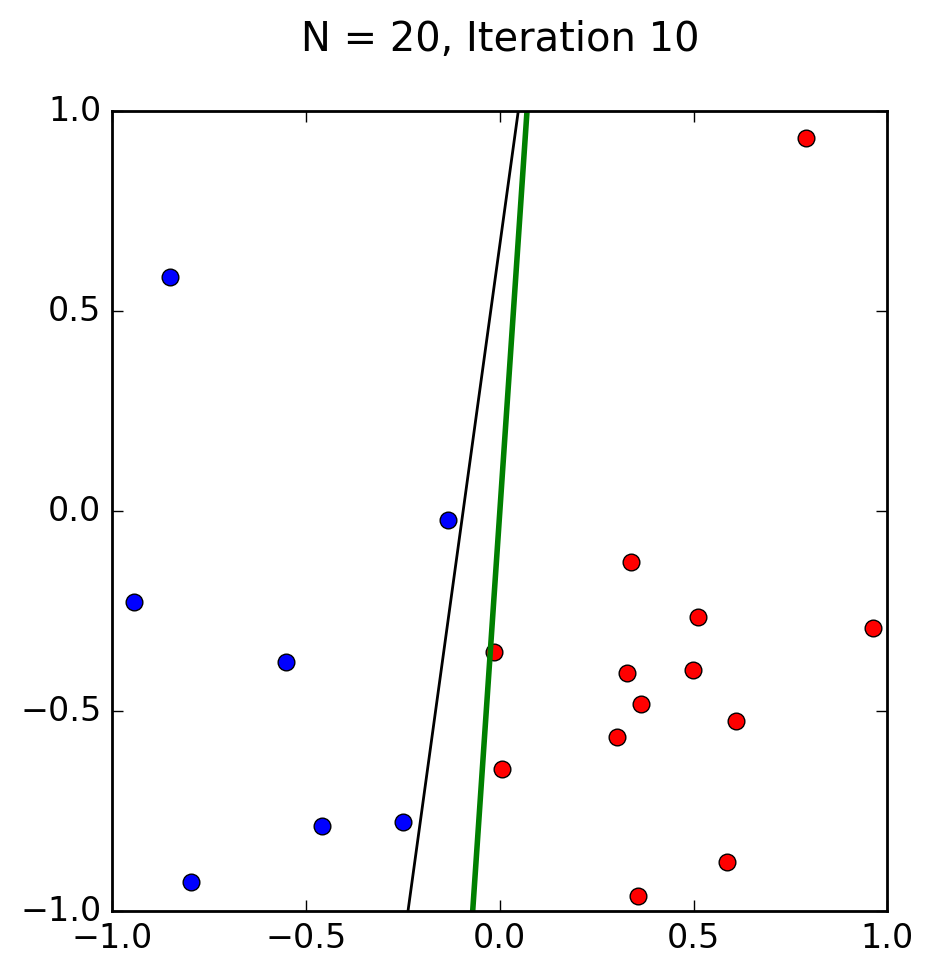
\includegraphics[width=9cm,height=9cm]{p_N20_it10.png}
  \caption{The final iteration of the perceptron learning algorithm using a different set of plot points.}
  \label{fig:PartC3}
\end{figure}

\subsection{Solution to Part D}
Part D states that we need to run the perceptron learning algorithm on a set of 100 points. Included are three iterations of the algorithm running. In the first picture, \ref{fig:PartD1}, the machine has gotten a start on finding f. The second picture, \ref{fig:PartD2}, has the g function nowhere near the target function, which is interesting considering this picture was 30 iterations later.  The last picture, \ref{fig:PartD3}, is when the algorithm stopped. Compared to both of the runs using 20 plot points, the finished hypothesis function is much closer to the target function, with only a small change in slope.  
\begin{figure}
  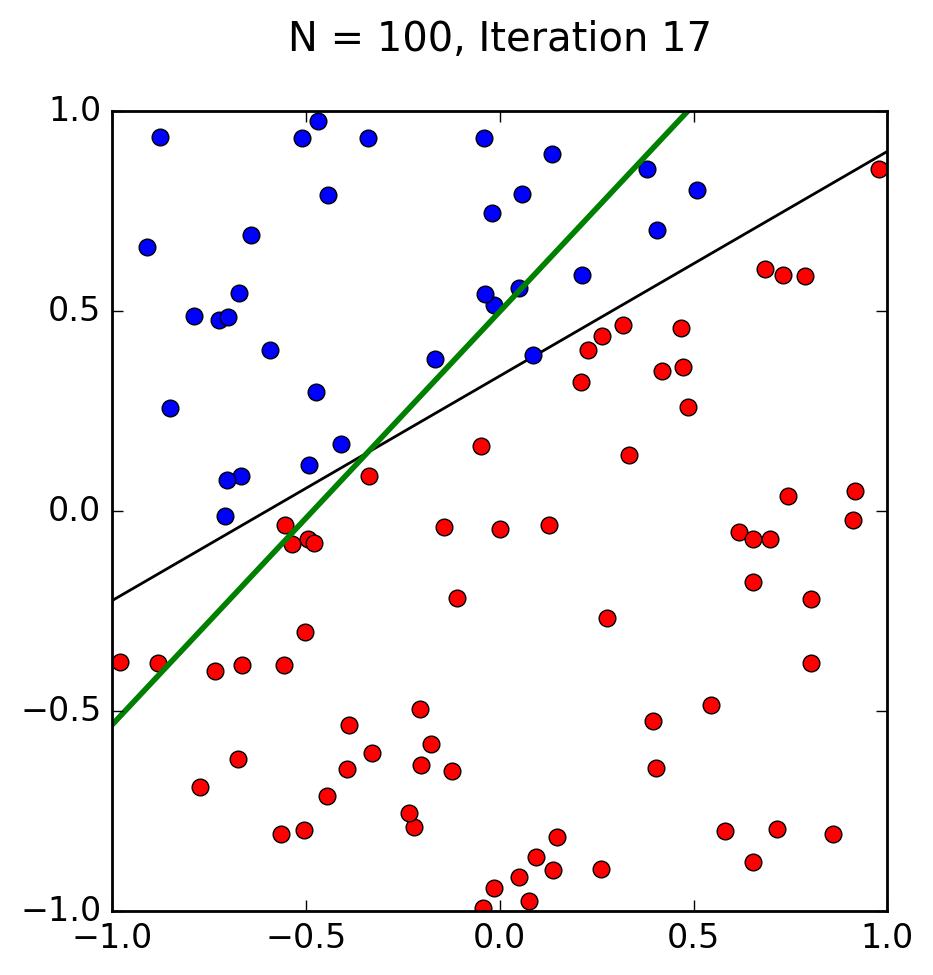
\includegraphics[width=9cm,height=9cm]{p_N100_it17.png}
  \caption{An iteration of the perceptron learning algorithm using 100 plot points.}
  \label{fig:PartD1}
\end{figure}
\begin{figure}
  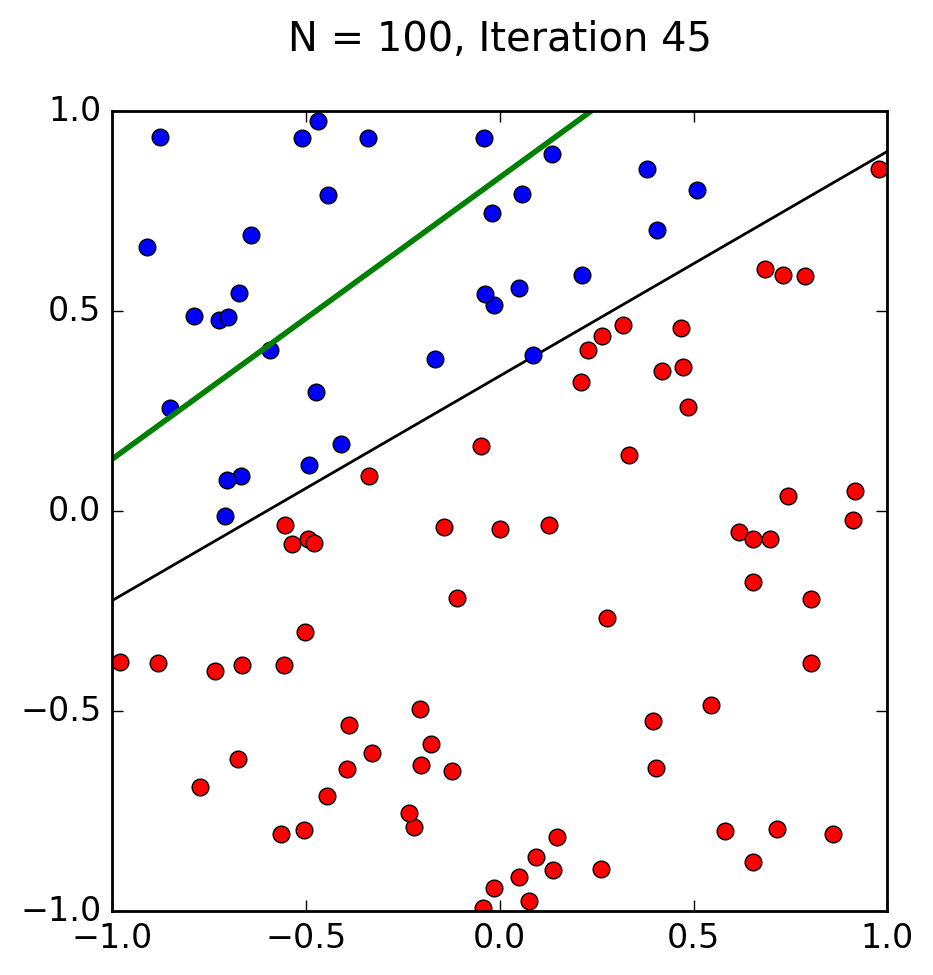
\includegraphics[width=9cm,height=9cm]{p_N100_it45.png}
  \caption{An iteration of the perceptron learning algorithm using 100 plot points.}
  \label{fig:PartD2}
\end{figure}
\begin{figure}
  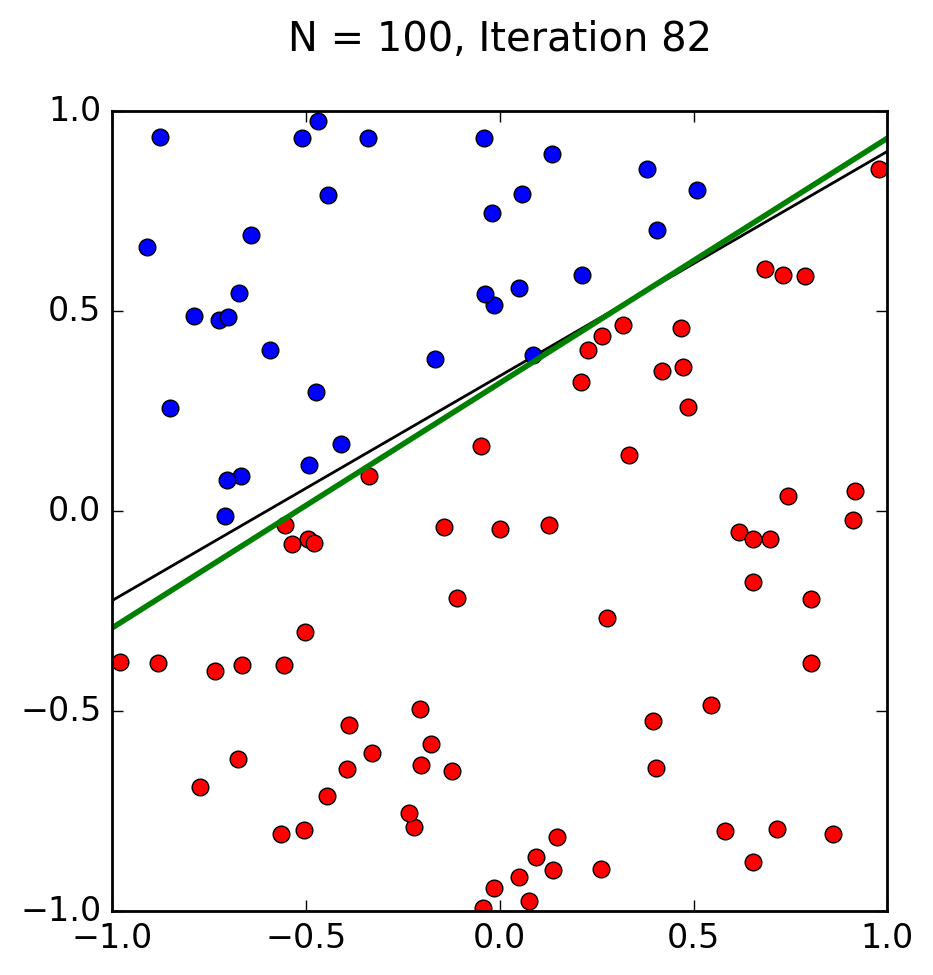
\includegraphics[width=9cm,height=9cm]{p_N100_it82.png}
  \caption{The final iteration of the perceptron learning algorithm using a set of 100 plot points.}
  \label{fig:PartD3}
\end{figure}

\subsection{Solution to Part E}
Part E states that we need to run the perceptron learning algorithm on a set of 1000 points. I hope my computer can handle this one.  Included are three iterations of the algorithm running. In the first picture, \ref{fig:PartE1}, the machine has gotten a start on finding f, and has no idea where it's going. The second picture, \ref{fig:PartE2}, has the g function much closer to the target function, but granted this is after the algorithm has done around 290 more iterations. The last picture, \ref{fig:PartE3}, is when the algorithm stopped, after exactly 332 iterations. If that's not nailing the target function, I don't know what is. Compared to both of the runs using 20 plot points and the 100 point one, the finished hypothesis function of this iteration is infinitely more accurate, to the point where I can't distinguish the target function from the hypothesis.
\begin{figure}
  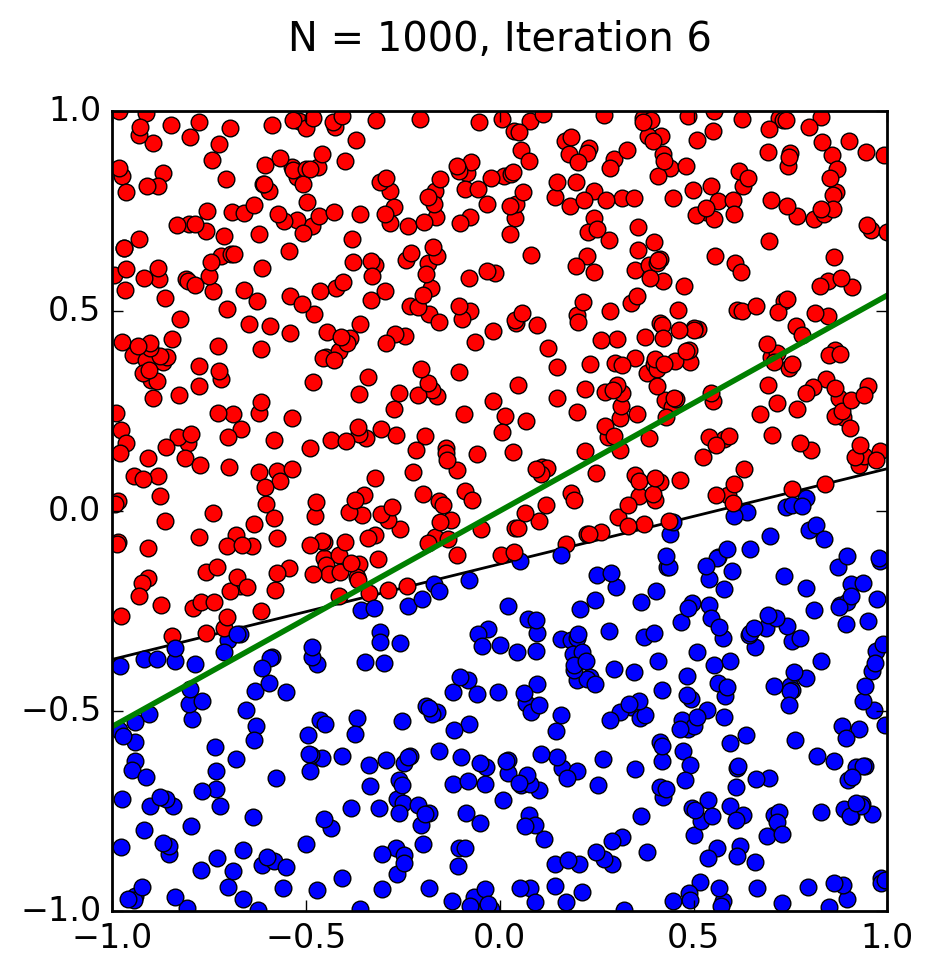
\includegraphics[width=9cm,height=9cm]{p_N1000_it6.png}
  \caption{An iteration of the perceptron learning algorithm using 1000 plot points.}
  \label{fig:PartE1}
\end{figure}
\begin{figure}
  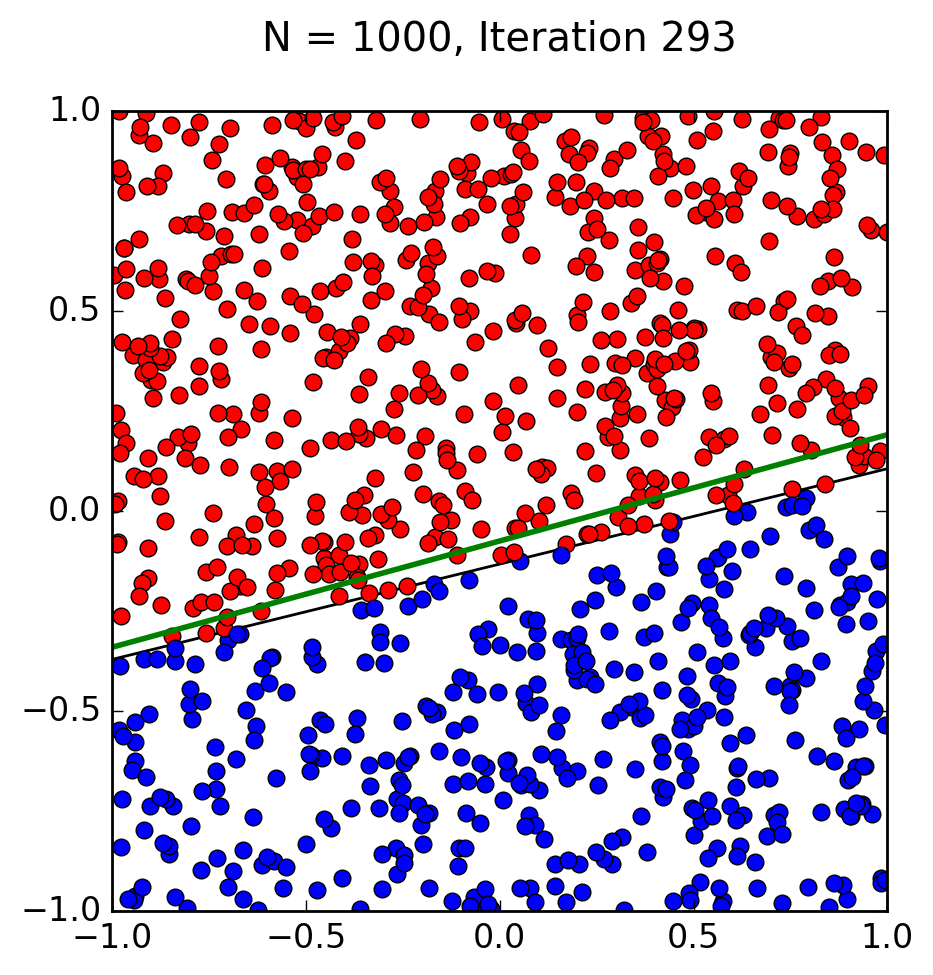
\includegraphics[width=9cm,height=9cm]{p_N1000_it293.png}
  \caption{An iteration of the perceptron learning algorithm using 1000 plot points.}
  \label{fig:PartE2}
\end{figure}
\begin{figure}
  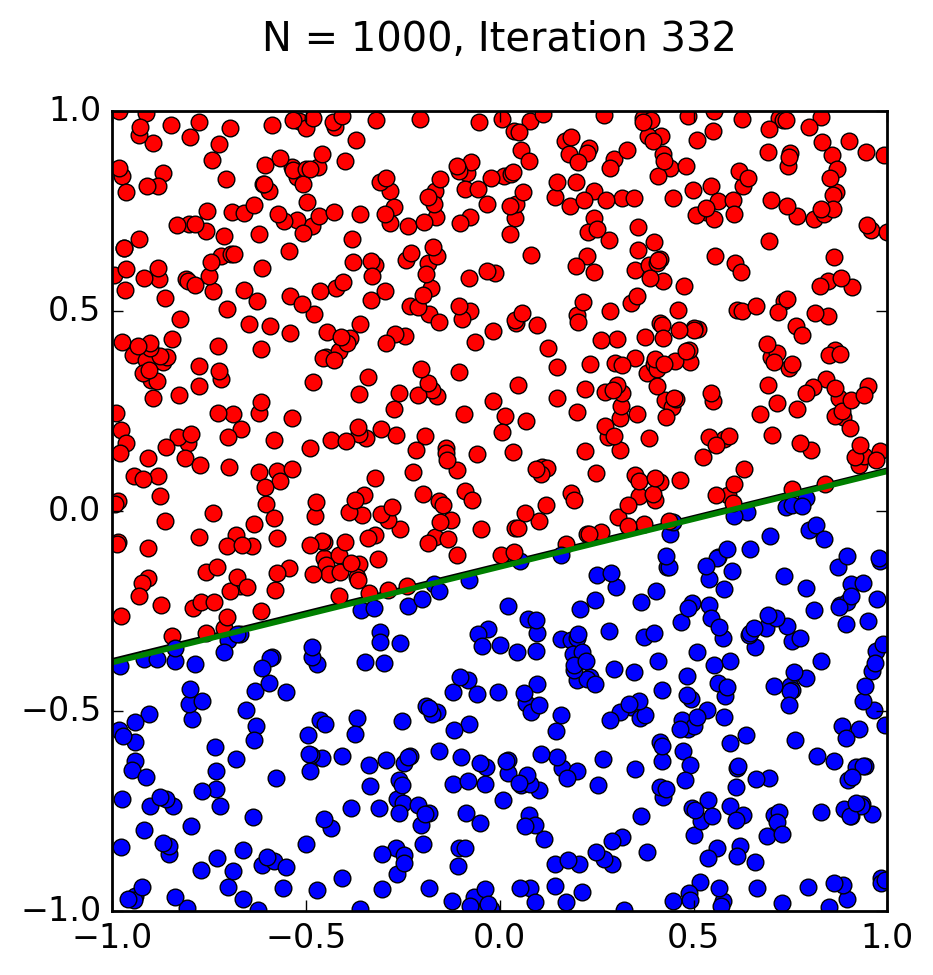
\includegraphics[width=9cm,height=9cm]{p_N1000_it332.png}
  \caption{The final iteration of the perceptron learning algorithm using a set of 1000 plot points.}
  \label{fig:PartE3}
\end{figure}

\subsection{Solution to Part F}
Part F needs us to edit the algorithm to fit 10 dimensions. I edited the code to use the random option. This file is found in Perceptron10.py. I ran the pla method once, and after 8266 updates, the algorithm stopped. What have I got myself into? Proof is in Figure \ref{fig:PartF}.

\begin{figure}
  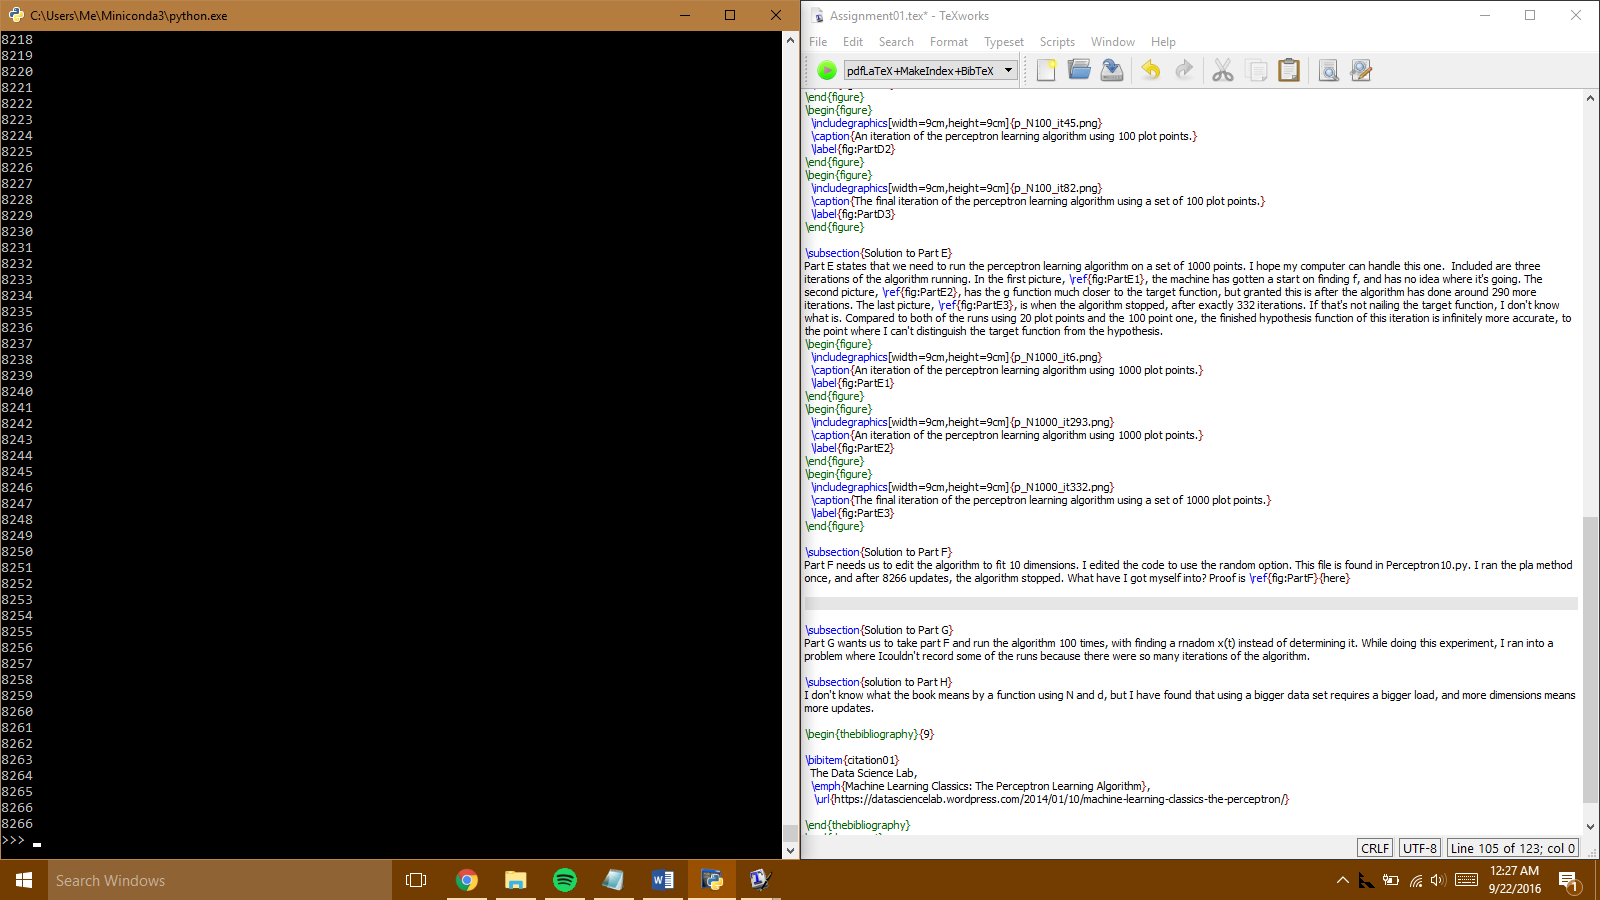
\includegraphics[width=9cm,height=9cm]{10DimensionConvergence.png}
  \caption{The final iteration using a set of 1000 plot points from 10 Dimensions(!), and LaTeX on the right.}
  \label{fig:PartF}
\end{figure}

\subsection{Solution to Part G}
Part G wants us to take part F and run the algorithm 100 times, with finding a random x(t) instead of determining it. To do this, I created the plaloop method, because i didn't want to hit the enter key 100 times. After a trip to McDonald's, the algorithm finished. The plot of point can be seen in this figure \ref{fig:PartG}.

\begin{figure}
  \includegraphics[width=9cm,height=9cm]{histogram.png}
  \caption{The results of running the perceptron learning algorithm with 1000 points 100 times. This took a while.}
  \label{fig:PartG}
\end{figure}

\subsection{solution to Part H}
I don't know what the book means by a function using N and d, but I have found that using a bigger data set requires a bigger load, and more dimensions means more updates.

\begin{thebibliography}{9}

\bibitem{citation01}
  The Data Science Lab,
  \emph{Machine Learning Classics: The Perceptron Learning Algorithm},
   \url{https://datasciencelab.wordpress.com/2014/01/10/machine-learning-classics-the-perceptron/}

\end{thebibliography}
\end{document}
